\documentclass[11pt,a4paper]{article}
\usepackage{amsmath}
\usepackage{amssymb}
\usepackage{enumitem}
\usepackage{amsthm}
\usepackage{listing}
\usepackage{MnSymbol}
\setlength{\parindent}{0pt}
\usepackage[utf8]{inputenc}
\usepackage{tikz}
\usepackage{listings} [python]
\usepackage{url}
\usepackage{xcolor}


\newtheorem{theorem}{Theorem}[section]
\newtheorem{corollary}{Corollary}[theorem]
\newtheorem{lemma}[theorem]{Lemma}
\newtheorem{mydef}{Definition}

%opening


%\newcommand{\imp}[1]{$\supset$}

\begin{document}



\section*{Exercise 1}
\begin{quote}
Prove, using splitting, that the formulas $p \leftrightarrow \neg q$ and  $\neg p \leftrightarrow q$ are equivalent.
\end{quote}
In order to show this one has to show that 
\begin{equation*}
\models (p \leftrightarrow \neg q) \leftrightarrow (\neg p \leftrightarrow q)
\end{equation*}
Unfortunately, splitting can only decide whether a formula is satisfiable or not. Hence, the problem 
\begin{equation*}
\nvDash \neg( (p \leftrightarrow \neg q) \leftrightarrow (\neg p \leftrightarrow q))
\end{equation*}
has to be considered. That is, if splitting applied to the formula above returns "unsatisfiable", it can be concluded that $(p \leftrightarrow \neg q) \leftrightarrow (\neg p \leftrightarrow q)$ is valid.


\begin{center}
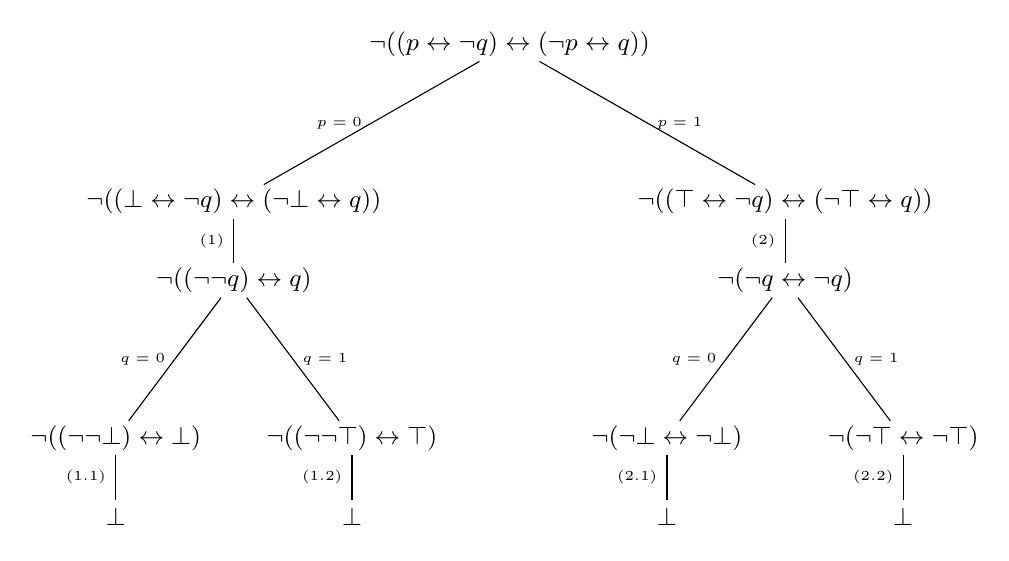
\begin{tikzpicture}
  \tikzset{vertex/.style = {shape=rectangle,minimum size=1.2em,inner sep=1pt}}
  \tikzset{edge/.style = {->,- = latex'}}

	\node[vertex] (0) at (5,12) {\small $\neg( (p \leftrightarrow \neg q) \leftrightarrow (\neg p \leftrightarrow q))$};
	
	
	\node[vertex] (1) at (1.5,10) {\small $\neg( (\bot \leftrightarrow \neg q) \leftrightarrow (\neg \bot \leftrightarrow q))$};

	\node[vertex] (11) at (1.5,9) {\small $\neg( (\neg \neg q) \leftrightarrow  q)$};
	
		\node[vertex] (111) at (0,7) {\small $\neg( (\neg \neg \bot) \leftrightarrow  \bot)$};
		\node[vertex] (1111) at (0,6) {\small $\bot$};
		
		\node[vertex] (112) at (3,7) {\small $\neg( (\neg \neg \top) \leftrightarrow \top)$};
		\node[vertex] (1121) at (3,6) {\small $\bot$};
		
		
	\node[vertex] (2) at (8.5,10) {\small $\neg( (\top \leftrightarrow \neg q) \leftrightarrow (\neg \top \leftrightarrow q))$};
		\node[vertex] (21) at (8.5,9) {\small $\neg (\neg q \leftrightarrow \neg q) $};
	
			\node[vertex] (211) at (7,7) {\small $\neg (\neg \bot \leftrightarrow \neg \bot) $};
			\node[vertex] (2111) at (7,6) {\small $\bot$};
			\node[vertex] (212) at (10,7) {\small $\neg (\neg \top \leftrightarrow \neg \top) $};
			\node[vertex] (2121) at (10,6) {\small $\bot$};
			
    \foreach \from/\to/\pos/\text in {0/1/left/$p=0$,0/2/right/$p=1$,1/11/left/$(1)$,11/111/left/$q=0$, 11/112/right/$q=1$, 111/1111/left/$(1.1)$, 112/1121/left/$(1.2)$, 2/21/left/$(2)$,21/211/left/$q=0$,21/212/right/$q=1$,211/2111/left/$(2.1)$,212/2121/left/$(2.2)$}
    \path[-](\from) edge node [\pos]{\tiny \text} (\to);
    
\end{tikzpicture}
\end{center}

With the respective transformations:
\begin{itemize} 
\item for $(1)$
\begin{equation*}
\begin{split}
&\neg( (\bot \leftrightarrow \neg q) \leftrightarrow (\neg \bot \leftrightarrow q)) \stackrel{\neg \bot \Rightarrow\top}{\longmapsto} 
\neg( (\bot \leftrightarrow \neg q) \leftrightarrow (\top \leftrightarrow q)) \\ 
&\stackrel{\bot \leftrightarrow A  \Rightarrow \neg A}{\longmapsto}
\neg( (\neg \neg q) \leftrightarrow (\top \leftrightarrow q)) \stackrel{\top \leftrightarrow A  \Rightarrow  A}{\longmapsto} \neg( (\neg \neg q) \leftrightarrow q)
\end{split}
\end{equation*}

\item for $(1.1)$
\begin{equation*}
\begin{split}
& \neg( (\neg \neg \bot) \leftrightarrow \bot) \stackrel{A \leftrightarrow \bot  \Rightarrow \neg A}{\longmapsto} \neg ( \neg \neg \neg \bot) \stackrel{\neg \bot \Rightarrow \top}{\longmapsto}
\neg ( \neg \neg \top) \stackrel{\neg \top \Rightarrow \bot}{\longmapsto} \neg ( \neg \bot) \\
&\stackrel{\neg \bot \Rightarrow \top}{\longmapsto} \neg \top \stackrel{\neg \top \Rightarrow \bot}{\longmapsto}
 \bot
\end{split}
\end{equation*}

\item for $(1.2)$
\begin{equation*}
\begin{split}
& \neg( (\neg \neg \top) \leftrightarrow \top) \stackrel{A \leftrightarrow \top  \Rightarrow A}{\longmapsto}
 \neg(\neg \neg \top) \stackrel{\neg \top \Rightarrow \bot}{\longmapsto}  \neg(\neg \bot) \stackrel{\neg \bot \Rightarrow \top}{\longmapsto}  \neg\top \stackrel{\neg \top \Rightarrow \bot}{\longmapsto}  \bot 
\end{split}
\end{equation*}

\item for $(2)$
\begin{equation*}
\begin{split}
&\neg( (\top \leftrightarrow \neg q) \leftrightarrow (\neg \top \leftrightarrow q)) \stackrel{\neg \top \Rightarrow\bot}{\longmapsto} 
\neg( (\top \leftrightarrow \neg q) \leftrightarrow (\bot \leftrightarrow q)) \\
&\stackrel{\top \leftrightarrow A \Rightarrow A}{\longmapsto} 
\neg(  \neg q \leftrightarrow (\bot \leftrightarrow q)) \stackrel{\bot \leftrightarrow A \Rightarrow \neg A}{\longmapsto} 
\neg(  \neg q \leftrightarrow \neg q) 
\end{split}
\end{equation*}
\item for $(2.1)$
\begin{equation*}
\begin{split}
& \neg(  \neg \bot \leftrightarrow \neg \bot)  \stackrel{\neg \bot \Rightarrow \top}{\longmapsto} 
\neg( \top \leftrightarrow \neg \bot)  \stackrel{\top \leftrightarrow A  \Rightarrow A}{\longmapsto}
\neg( \neg \bot)  \stackrel{\neg \bot \Rightarrow \top}{\longmapsto} 
\neg \top \stackrel{\neg \top \Rightarrow \bot}{\longmapsto} 
 \bot
\end{split}
\end{equation*}

\item for $(2.2)$
\begin{equation*}
\begin{split}
& \neg(  \neg \top \leftrightarrow \neg \top)  \stackrel{\neg \top \Rightarrow \top}{\longmapsto} 
\neg( \bot \leftrightarrow \neg \bot)  \stackrel{\bot \leftrightarrow A  \Rightarrow \neg A}{\longmapsto}
\neg( \neg \neg \top)  \stackrel{\neg \top \Rightarrow \bot}{\longmapsto} 
\neg( \neg\bot) \\
& \stackrel{\neg \bot \Rightarrow \top}{\longmapsto} 
\neg \top \stackrel{\neg \top \Rightarrow \bot}{\longmapsto} 
 \bot
\end{split}
\end{equation*}
\end{itemize}


\section*{Exercise 2}
\begin{quote}
Apply the optimized definitional clausal transformation algorithm to the formula:
\begin{equation*}
\neg((p\leftrightarrow q) \leftrightarrow (r \leftrightarrow q))
\end{equation*}
Apply the DPLL algorithm to the resulting set of clauses. If the resulting set of clauses is satisfiable,
give a model of the formula above.
\end{quote}
By applying the optimised definitional clausal transformation algorithm one obtains the following 
\begin{center}
\begin{tabular}{| l | l | l | l | }
\hline
labels & subformulas & definitions & clauses \\
\hline
- & - & $n_1$ & $n_1$ \\
$n_1$ & $\neg((p\leftrightarrow q) \leftrightarrow (r \leftrightarrow q))$ & $n_1 \to \neg n_2$ & see (1) \\
$n_2$ & $\textcolor{white}{\neg(}(p\leftrightarrow q) \leftrightarrow (r \leftrightarrow q)\textcolor{white}{)}$  &  $(n_3 \leftrightarrow n_4) \to n_2$ & see (2) \\
$n_3$ & $\textcolor{white}{\neg(}(p\leftrightarrow q) \textcolor{white}{\leftrightarrow (r \leftrightarrow q))}$ & $n_3 \leftrightarrow (p \leftrightarrow q) $ & see (3) \\
$n_4$ & $\textcolor{white}{\neg((p\leftrightarrow q) \leftrightarrow} (r \leftrightarrow q)\textcolor{white}{)}$  & $n_4 \leftrightarrow (r \leftrightarrow q) $  & see (4)\\
\hline
\end{tabular}
\end{center}
(Note that $n_1$ only occurs positively, $n_2$ only negatively and the other have no polarity)\\


From there the definitions must be transformed into CNF (some steps are skipped to decrease the amount of depicted transformations). 
\begin{itemize}
\item (1) is $\neg n_1 \lor \neg n_2$, because $n_1 \to \neg n_2 \mapsto \neg n_1 \lor \neg n_2$ 
\item (2) is $(n_3 \lor n_4 \lor n_2) \land (n_3 \lor \neg  n_3 \lor n_2) \land (\neg n_4 \lor  n_4 \lor n_2) \land(\neg n_4 \lor  \neg  n_3 \lor n_2)$, because $(n_3 \leftrightarrow n_4) \to n_2 \mapsto \neg (n_3 \leftrightarrow n_4) \lor n_2 \mapsto \neg ((\neg n_3 \lor n_4) \land (\neg n_4 \lor n_3)) \lor n_2 \mapsto \neg (\neg n_3 \lor n_4) \lor \neg (\neg n_4 \lor n_3) \lor n_2 \mapsto  (n_3 \land \neg n_4) \lor  (n_4 \land\neg  n_3) \lor n_2 \mapsto  (n_3 \lor  (n_4 \land\neg  n_3) \land (\neg n_4 \lor  (n_4 \land\neg  n_3))  \lor n_2  \mapsto  ((n_3 \lor n_4) \land (n_3 \lor \neg  n_3) \land (\neg n_4 \lor  n_4) \land(\neg n_4 \lor  \neg  n_3))  \lor n_2 \mapsto  (n_3 \lor n_4 \lor n_2) \land (n_3 \lor \neg  n_3 \lor n_2) \land (\neg n_4 \lor  n_4 \lor n_2) \land(\neg n_4 \lor  \neg  n_3 \lor n_2)$ 
\item (3) is $(\neg n_3 \lor \neg p \lor q) \land (\neg n_3 \lor \neg q \lor p) \land (p\lor q \lor n_3)\land (p \lor \neg p \lor n_3) \land (\neg q \lor q \lor n_3)\land (\neg q \lor \neg p \lor n_3)$, because  $n_3 \leftrightarrow (p \leftrightarrow q) \mapsto (\neg n_3 \lor (p \leftrightarrow q)) \land (\neg (p \leftrightarrow q) \lor n_3) \mapsto (\neg n_3 \lor ((\neg p \lor q) \land (\neg q \lor p)) \land (\neg (p \leftrightarrow q) \lor n_3) \mapsto (\neg n_3 \lor \neg p \lor q) \land (\neg n_3 \lor \neg q \lor p) \land (\neg (p \leftrightarrow q) \lor n_3) \mapsto (\neg n_3 \lor \neg p \lor q) \land (\neg n_3 \lor \neg q \lor p) \land (\neg ((\neg p \lor q) \land (\neg q \lor p)) \lor n_3)$ from there after a sequence of transformations as in (2) one obtains $(\neg n_3 \lor \neg p \lor q) \land (\neg n_3 \lor \neg q \lor p) \land (p\lor q \lor n_3)\land (p \lor \neg p \lor n_3) \land (\neg q \lor q \lor n_3)\land (\neg q \lor \neg p \lor n_3)$

\item (4) is $(\neg n_4 \lor \neg r \lor q) \land (\neg n_4 \lor \neg q \lor r) \land (r \lor q \lor n_4)\land (r \lor \neg r \lor n_4) \land (\neg q \lor q \lor n_4)\land (\neg q \lor \neg r \lor n_4)$, because of the same sequence of transformations as in (3).
\end{itemize}

Hence, we obtain the following set of clauses.

\begin{align*}
&(n_1),& & (\neg n_3 \lor \neg p \lor q), & & (\neg n_4 \lor \neg r \lor q),\\ 
&(\neg n_1 \lor \neg n_2),& & (\neg n_3 \lor \neg q \lor p),  && (\neg n_4 \lor \neg q \lor r), \\
&(n_3 \lor n_4 \lor n_2),& & (p\lor q \lor n_3),  && (r \lor q \lor n_4), \\
&(n_3 \lor \neg  n_3 \lor n_2) ,  & & (p \lor \neg p \lor n_3), & & (r \lor \neg r \lor n_4), \\
&(\neg n_4 \lor  n_4 \lor n_2) , & & (\neg q \lor q \lor n_3),& & (\neg q \lor q \lor n_4), \\
&(\neg n_4 \lor  \neg  n_3 \lor n_2), && (\neg q \lor \neg p \lor n_3), & & (\neg q \lor \neg r \lor n_4)
\end{align*}

%Now by applying the two optimisations one obtains 
%
%\begin{align*}
%&(\neg n_1 \lor \neg n_2), & & (\neg n_3 \lor \neg p \lor q), & & (\neg n_4 \lor \neg r \lor q),\\ 
%&(n_3 \lor n_4 \lor n_2), & & (\neg n_3 \lor \neg q \lor p),  && (\neg n_4 \lor \neg q \lor r), \\
%&(n_3 \lor \neg  n_3 \lor n_2) , & & (p\lor q \lor n_3),  && (r \lor q \lor n_4), \\
%&(\neg n_4 \lor  n_4 \lor n_2) , & & (p \lor \neg p \lor n_3), & & (r \lor \neg r \lor n_4), \\
%&(\neg n_4 \lor  \neg  n_3 \lor n_2),& & (\neg q \lor q \lor n_3),& & (\neg q \lor q \lor n_4), \\
%& && (\neg q \lor \neg p \lor n_3), & & (\neg q \lor \neg r \lor n_4)
%\end{align*}
Taking this set of clauses as input for DPLL one can observe the following sequence of events. However, this is not the only possible sequence of events, as the choice of literal is non-deterministic. That is, while the algorithm normally creates a tree, we were lucky and the initial choices of literals already showed satisfiability. Hence, due to the depth first search tactic of DPLL the algorithm only had to investigate a path within the search space.

\begin{enumerate}

\item 
\begin{enumerate}
\item The clause set is:
\begin{align*}
&(n_1),& & (\neg n_3 \lor \neg p \lor q), & & (\neg n_4 \lor \neg r \lor q),\\ 
&(\neg n_1 \lor \neg n_2),& & (\neg n_3 \lor \neg q \lor p),  && (\neg n_4 \lor \neg q \lor r), \\
&(n_3 \lor n_4 \lor n_2),& & (p\lor q \lor n_3),  && (r \lor q \lor n_4), \\
&(n_3 \lor \neg  n_3 \lor n_2) ,  & & (p \lor \neg p \lor n_3), & & (r \lor \neg r \lor n_4), \\
&(\neg n_4 \lor  n_4 \lor n_2) , & & (\neg q \lor q \lor n_3),& & (\neg q \lor q \lor n_4), \\
&(\neg n_4 \lor  \neg  n_3 \lor n_2), && (\neg q \lor \neg p \lor n_3), & & (\neg q \lor \neg r \lor n_4)
\end{align*}
\item Unit clause exists. Propagate:
\begin{enumerate}
\item Unit Clause:  $n_1$
\begin{align*}
&\textcolor{red}{(n_1)},& & (\neg n_3 \lor \neg p \lor q), & & (\neg n_4 \lor \neg r \lor q),\\ 
&(\textcolor{red}{\neg n_1} \lor \neg n_2),& & (\neg n_3 \lor \neg q \lor p),  && (\neg n_4 \lor \neg q \lor r), \\
&(n_3 \lor n_4 \lor n_2),& & (p\lor q \lor n_3),  && (r \lor q \lor n_4), \\
&(n_3 \lor \neg  n_3 \lor n_2) ,  & & (p \lor \neg p \lor n_3), & & (r \lor \neg r \lor n_4), \\
&(\neg n_4 \lor  n_4 \lor n_2) , & & (\neg q \lor q \lor n_3),& & (\neg q \lor q \lor n_4), \\
&(\neg n_4 \lor  \neg  n_3 \lor n_2), && (\neg q \lor \neg p \lor n_3), & & (\neg q \lor \neg r \lor n_4)
\end{align*}
\item Unit Clause:  $\neg n_2$
\begin{align*}
& & & (\neg n_3 \lor \neg p \lor q), & & (\neg n_4 \lor \neg r \lor q),\\ 
&\textcolor{red}{(\neg n_2)},& & (\neg n_3 \lor \neg q \lor p),  && (\neg n_4 \lor \neg q \lor r), \\
&(n_3 \lor n_4 \lor \textcolor{red}{n_2}),& & (p\lor q \lor n_3),  && (r \lor q \lor n_4), \\
&(n_3 \lor \neg  n_3 \lor \textcolor{red}{n_2}) ,  & & (p \lor \neg p \lor n_3), & & (r \lor \neg r \lor n_4), \\
&(\neg n_4 \lor  n_4 \lor \textcolor{red}{n_2}) , & & (\neg q \lor q \lor n_3),& & (\neg q \lor q \lor n_4), \\
&(\neg n_4 \lor  \neg  n_3 \lor \textcolor{red}{n_2}), && (\neg q \lor \neg p \lor n_3), & & (\neg q \lor \neg r \lor n_4)
\end{align*}
\end{enumerate}
\item The clause set is not empty.
\item The clause set does not contain the empty clause.
\item Select literal: $n_3$
\end{enumerate}




\item 
\begin{enumerate}
\item The clause set is:
\begin{align*}
& & & (\neg n_3 \lor \neg p \lor q), & & (\neg n_4 \lor \neg r \lor q),\\ 
& (n_3) & & (\neg n_3 \lor \neg q \lor p),  && (\neg n_4 \lor \neg q \lor r), \\
&(n_3 \lor n_4),& & (p\lor q \lor n_3),  && (r \lor q \lor n_4), \\
&(n_3 \lor \neg  n_3 ) ,  & & (p \lor \neg p \lor n_3), & & (r \lor \neg r \lor n_4), \\
&(\neg n_4 \lor  n_4 ) , & & (\neg q \lor q \lor n_3),& & (\neg q \lor q \lor n_4), \\
&(\neg n_4 \lor  \neg  n_3), && (\neg q \lor \neg p \lor n_3), & & (\neg q \lor \neg r \lor n_4)
\end{align*}
\item Unit clause exists. Propagate:
\begin{enumerate}
\item Unit Clause:  $n_3$
\begin{align*}
& & & (\textcolor{red}{\neg n_3} \lor \neg p \lor q), & & (\neg n_4 \lor \neg r \lor q),\\ 
& \textcolor{red}{(n_3)} & & (\textcolor{red}{\neg n_3} \lor \neg q \lor p),  && (\neg n_4 \lor \neg q \lor r), \\
&\textcolor{red}{(n_3 \lor n_4)},& & \textcolor{red}{(p\lor q \lor n_3)},  && (r \lor q \lor n_4), \\
&\textcolor{red}{(n_3 \lor \neg  n_3 )} ,  & & \textcolor{red}{(p \lor \neg p \lor n_3)}, & & (r \lor \neg r \lor n_4), \\
&(\neg n_4 \lor  n_4 ) , & &\textcolor{red}{(\neg q \lor q \lor n_3)},& & (\neg q \lor q \lor n_4), \\
&(\neg n_4 \lor  \textcolor{red}{\neg  n_3}), && \textcolor{red}{(\neg q \lor \neg p \lor n_3)}, & & (\neg q \lor \neg r \lor n_4)
\end{align*}
\item Unit Clause:  $\neg n_4$
\begin{align*}
& & & ( \neg p \lor q), & & \textcolor{red}{(\neg n_4 \lor \neg r \lor q)},\\ 
& & & (\neg q \lor p),  && \textcolor{red}{(\neg n_4 \lor \neg q \lor r)}, \\
& & &  && (r \lor q \lor \textcolor{red}{n_4}), \\
& & &  & & (r \lor \neg r \lor \textcolor{red}{n_4}), \\
&\textcolor{red}{(\neg n_4 \lor  n_4 )} , & & & & (\neg q \lor q \lor \textcolor{red}{n_4}), \\
&\textcolor{red}{(\neg n_4 )}, &&  & & (\neg q \lor \neg r \lor \textcolor{red}{ n_4})
\end{align*}
\end{enumerate}
\item The clause set is not empty.
\item The clause set does not contain the empty clause.
\item Select literal: $\neg p$
\end{enumerate}



\item 
\begin{enumerate}
\item The clause set is:
\begin{align*}
&( \neg p ), \\ 
&( \neg p \lor q), \\ 
&(\neg q \lor p), \\
&(r \lor q), \\
&(r \lor \neg r ), \\
&(\neg q \lor q ), \\
&(\neg q \lor \neg r)
\end{align*}
\item Unit clause exists. Propagate:
\begin{enumerate}
\item Unit Clause:  $\neg p$
\begin{align*}
&\textcolor{red}{( \neg p )}, \\ 
&\textcolor{red}{( \neg p \lor q)}, \\ 
&(\neg q \lor \textcolor{red}{p}), \\
&(r \lor q), \\
&(r \lor \neg r ), \\
&(\neg q \lor q ), \\
&(\neg q \lor \neg r)
\end{align*}
\item Unit Clause:  $\neg q$
\begin{align*}
&\textcolor{red}{(\neg q )}, \\
&(r \lor \textcolor{red}{q}), \\
&(r \lor \neg r ), \\
&\textcolor{red}{(\neg q \lor q )}, \\
&\textcolor{red}{(\neg q \lor \neg r)}
\end{align*}
\item Unit Clause:  $r$
\begin{align*}
&\textcolor{red}{(r )}, \\
&\textcolor{red}{(r \lor \neg r )} \\
\end{align*}
\end{enumerate}
\item The clause set is empty. Return \emph{satisfiable}.
\end{enumerate}

\end{enumerate}

This is only one path in the whole DPLL tree. If this selection of literals would have resulted in the empty clause one would need to consider further branches of the DPLL tree. Given this path the following literals were chosen during unit propagation $n_1, \neg n_2, n_3, \neg n_4, \neg p, \neg q, r$. Hence, resulting in the interpretation $\{n_1 \mapsto 1, n_2 \mapsto 0, n_3 \mapsto 1, n_4 \mapsto 0, p \mapsto 0, q \mapsto 0, r\mapsto 1\}$. Lastly, having found one interpretation, further investigation of the DPLL tree is not required.\\



If one chooses to apply the two optimisations before applying DPLL, one has to remove the tautologies

\begin{align*}
& (n_1)& & (\neg n_3 \lor \neg p \lor q), & & (\neg n_4 \lor \neg r \lor q),\\ 
&(\neg n_1 \lor \neg n_2),  & & (\neg n_3 \lor \neg q \lor p),  && (\neg n_4 \lor \neg q \lor r), \\
&(n_3 \lor n_4 \lor n_2), & & (p\lor q \lor n_3),  && (r \lor q \lor n_4), \\
&\textcolor{red}{(n_3 \lor \neg  n_3 \lor n_2)} , & & \textcolor{red}{(p \lor \neg p \lor n_3)}, & & \textcolor{red}{(r \lor \neg r \lor n_4)}, \\
& \textcolor{red}{(\neg n_4 \lor  n_4 \lor n_2)} , & & \textcolor{red}{(\neg q \lor q \lor n_3)},& & \textcolor{red}{(\neg q \lor q \lor n_4)}, \\
&(\neg n_4 \lor  \neg  n_3 \lor n_2), && (\neg q \lor \neg p \lor n_3), & & (\neg q \lor \neg r \lor n_4)
\end{align*}

as well as the clauses with pure literals. However, in this case there are none. From there this reduced set of clauses serves as input for DPLL, producing a computation similar to the one above.


\section*{Exercise 3}

\begin{center}
\begin{tikzpicture}
  \tikzset{vertex/.style = {shape=rectangle,minimum size=1.2em,inner sep=1pt}}
  \tikzset{edge/.style = {->,- = latex'}}

	\node[vertex] (0) at (5,9) {\small $\land^{[+]}$};
	
	\node[vertex] (1) at (1,8) {\small $\to^{[+]}$};
	
		\node[vertex] (2) at (0,7) {\small $p^{[-]}$};
	
		\node[vertex] (3) at (3,7) {\small $\land^{[+]}$};
		
			\node[vertex] (4) at (2,6) {\small $\neg^{[+]}$};
			\node[vertex] (5) at (2,5) {\small $q^{[-]}$};
			
			\node[vertex] (6) at (4,6) {\small $r^{[+]}$};
	
	\node[vertex] (7) at (7,8) {\small $\lor^{[+]}$};
		
		\node[vertex] (8) at (6,7) {\small $p^{[+]}$};
		
		\node[vertex] (9) at (9,7) {\small $\to^{[+]}$};
		
			\node[vertex] (10) at (8,6) {\small $q^{[-]}$};
			
			\node[vertex] (11) at (11,6) {\small $\lor^{[+]}$};
			
				\node[vertex] (12) at (10,5) {\small $r^{[+]}$};
				
				\node[vertex] (13) at (12,5) {\small $p^{[+]}$};
	
			
    \foreach \from/\to/\pos/\text in {0/1/left/$1$,1/2/right/$1$,1/3/right/$2$,
    3/4/right/$1$,4/5/right/$2$,3/6/right/$2$,0/7/right/$2$,7/8/right/$1$,7/9/right/$2$,
    9/10/right/$1$,9/11/right/$2$,11/12/right/$1$,11/13/right/$2$
    }
    \path[-](\from) edge node [\pos]{\tiny \text} (\to);
    
\end{tikzpicture}
\end{center}
Since, $q$ only has negative polarity it is anti-monotonic. Moreover, the only occurrence $r$ is positive, thus $r$ is monotonic. Lastly, $p$ occurs positively as well as negatively, thus $p$ is neither monotonic nor anti-monotonic.


\begin{center}
\begin{tabular}{| l | l | l | l | }
\hline
labels & subformulas & definitions & clauses \\
\hline
- & - & $n_1$ & $n_1$ \\
$n_1$ & $(p \to (\neg q \land r)) \land (p \lor (q \to (r \lor p)))$ & $n_1 \to (n_2 \land n_4) $ & see (1) \\
$n_2$ & $(p \to (\neg q \land r)) \textcolor{white}{\land (p \lor (q \to (r \lor q)))}$ & $n_2 \to (p \to n_3) $ & see (2) \\
$n_3$ & $\textcolor{white}{(p \to} \;(\neg q \land r)\textcolor{white}{) \land (p \lor (q \to (r \lor q)))}$ & $ n_3 \to (\neg q \land r)$ & see (3)\\
$n_4$ & $\textcolor{white}{(p \to (\neg q \land r)) \land }(p \lor (q \to (r \lor p)))$ & $n_4 \to (p \lor n_5) $ & see (4)\\
$n_5$ & $\textcolor{white}{(p \to (\neg q \land r)) \land (p \lor }(q \to (r \lor p))\textcolor{white}{)}$ & $n_5 \to (q \to n_6)$ & see (5)\\
$n_6$ & $\textcolor{white}{(p \to (\neg q \land r)) \land (p \lor (q \to} (r \lor p)\textcolor{white}{))}$ & $n_6 \to (r \lor p) $ & see (6) \\
\hline
\end{tabular}
\end{center}
(Note that all subformulas occur positively)


\begin{itemize}
\item (1) is $(\neg n_1 \lor n_2 )\land (\neg  n_1 \lor n_4) $, because $n_1 \to (n_2 \land n_4)  \mapsto \neg n_1 \lor (n_2 \land n_4) \mapsto \neg n_1 \lor n_2 \land \neg  n_1 \lor n_4$;
\item (2) is $\neg n_2 \lor \neg p \lor n_3 $, because $n_2 \to (p \to n_3) \mapsto \neg n_2 \lor (p \to n_3) \mapsto \neg n_2 \lor \neg p \lor n_3$;
\item (3) is $(\neg n_3 \lor \neg q) \land (\neg n_3 \lor r)$, because $n_3 \to (\neg q \land r) \mapsto \neg n_3 \lor (\neg q \land r) \mapsto\neg  n_3 \lor \neg q \land \neg n_3 \lor r$;
\item (4) is $\neg n_4 \lor p \lor n_5$, because $n_4 \to (p \lor n_5) \mapsto \neg n_4 \lor p \lor n_5$;
\item (5) is $\neg n_5 \lor \neg q \lor n_6$, because $n_5 \to (q \to n_6) \mapsto \neg n_5 \lor (q \to n_6) \mapsto  \neg n_5 \lor \neg q \lor n_6$;
\item (6) is $\neg n_6 \lor r \lor p$, because $n_6 \to (r \lor p) \mapsto \neg n_6 \lor r \lor p$
\end{itemize}


Hence, one obtains the following set of clauses.
\begin{align*}
& (n_1) \\
& (\neg n_1 \lor n_2 ), &&  (\neg  n_1 \lor n_4), \\
& (\neg n_2 \lor \neg p \lor n_3), \\
& (\neg n_3 \lor \neg q) , &&  (\neg n_3 \lor r), \\
& (\neg n_4 \lor p \lor n_5), \\
& (\neg n_5 \lor \neg q \lor n_6), \\
& (\neg n_6 \lor r \lor p)
\end{align*}



\begin{enumerate}

\item 
\begin{enumerate}
\item The clause set is:
\begin{align*}
& (n_1) \\
& (\neg n_1 \lor n_2 ), &&  (\neg  n_1 \lor n_4), \\
& (\neg n_2 \lor \neg p \lor n_3), \\
& (\neg n_3 \lor \neg q) , &&  (\neg n_3 \lor r), \\
& (\neg n_4 \lor p \lor n_5), \\
& (\neg n_5 \lor \neg q \lor n_6), \\
& (\neg n_6 \lor r \lor p)
\end{align*}
\item Unit clause exists. Propagate:
\begin{enumerate}
\item Unit Clause:  $n_1$
\begin{align*}
& \textcolor{red}{(n_1)} \\
& (\textcolor{red}{\neg n_1} \lor n_2 ), &&  (\textcolor{red}{\neg  n_1} \lor n_4), \\
& (\neg n_2 \lor \neg p \lor n_3), \\
& (\neg n_3 \lor \neg q) , &&  (\neg n_3 \lor r), \\
& (\neg n_4 \lor p \lor n_5), \\
& (\neg n_5 \lor \neg q \lor n_6), \\
& (\neg n_6 \lor r \lor p)
\end{align*}
\item Unit Clause:  $n_2$
\begin{align*}
& \textcolor{red}{(n_2)}, &&  (n_4), \\
& (\textcolor{red}{\neg n_2} \lor \neg p \lor n_3), \\
& (\neg n_3 \lor \neg q) , &&  (\neg n_3 \lor r), \\
& (\neg n_4 \lor p \lor n_5), \\
& (\neg n_5 \lor \neg q \lor n_6), \\
& (\neg n_6 \lor r \lor p)
\end{align*}
\item Unit Clause:  $n_4$
\begin{align*}
& (\neg p \lor n_3), &&  \textcolor{red}{(n_4)},\\
& (\neg n_3 \lor \neg q) , &&  (\neg n_3 \lor r), \\
& (\textcolor{red}{\neg n_4} \lor p \lor n_5), \\
& (\neg n_5 \lor \neg q \lor n_6), \\
& (\neg n_6 \lor r \lor p)
\end{align*}
\end{enumerate}
\item The clause set is not empty.
\item The clause set does not contain the empty clause.
\item Select literal: $n_3$
\end{enumerate}


\item 
\begin{enumerate}
\item The clause set is:
\begin{align*}
& (n_3), \\
& (\neg p \lor n_3), \\
& (\neg n_3 \lor \neg q) , &&  (\neg n_3 \lor r), \\
& ( p \lor n_5), \\
& (\neg n_5 \lor \neg q \lor n_6), \\
& (\neg n_6 \lor r \lor p)
\end{align*}
\item Unit clause exists. Propagate:
\begin{enumerate}
\item Unit Clause:  $n_3$
\begin{align*}
& \textcolor{red}{(n_3)}, \\
& \textcolor{red}{(\neg p \lor n_3)}, \\
& (\textcolor{red}{\neg n_3} \lor \neg q) , &&  (\textcolor{red}{\neg n_3} \lor r), \\
& ( p \lor n_5), \\
& (\neg n_5 \lor \neg q \lor n_6), \\
& (\neg n_6 \lor r \lor p)
\end{align*}
\item Unit Clause:  $\neg q$
\begin{align*}
& \textcolor{red}{(\neg q)} , &&  (r), \\
& ( p \lor n_5), \\
& \textcolor{red}{(\neg n_5 \lor \neg q \lor n_6)}, \\
& (\neg n_6 \lor r \lor p)
\end{align*}
\item Unit Clause:  $r$
\begin{align*}
& \textcolor{red}{(r)}, \\
& ( p \lor n_5), \\
& (\neg n_6 \lor \textcolor{red}{r} \lor p)
\end{align*}
%\item Unit Clause:  $\neg n_6$
%\begin{align*}
%& ( p \lor n_5), \\
%& \textcolor{red}{(\neg n_6 \lor ) }
%\end{align*}
\end{enumerate}
\item The clause set is not empty.
\item The clause set does not contain the empty clause.
\item Select literal: $p$
\end{enumerate}

\item 
\begin{enumerate}
\item The clause set is:
\begin{align*}
& (p) \\
& ( p \lor n_5) \\
& (\neg n_6 \lor p)
\end{align*}
\item Unit clause exists. Propagate:
\begin{enumerate}
\item Unit Clause:  $p$
\begin{align*}
& \textcolor{red}{(p)} \\
& \textcolor{red}{( p \lor n_5)} \\
& \textcolor{red}{(\neg n_6 \lor p)} \\
\end{align*}
\end{enumerate}
\item The clause set is empty. Return \emph{satisfiable}.
\end{enumerate}

\end{enumerate}
 Given this path the following literals were chosen during unit propagation $n_1, n_2, n_3, n_4, p, \neg q, r$. Since, $n_5$ and $n_6$ were not fixed, its truth value is inconsequential (given the fixed atoms). Hence, resulting in the interpretation $\{n_1 \mapsto 1, n_2 \mapsto 1, n_3 \mapsto 1, n_4 \mapsto 1, n_5 \mapsto 0, n_6 \mapsto 0, p \mapsto 1, q \mapsto 0, r\mapsto 1\}$. Lastly, having found one interpretation, further investigation of the DPLL tree is not required. \\




Alternatively, applying the optimisation rules. That is, remove all tautologies and all clauses with pure literals. There are no tautologies. Leaving the removal of clauses with pure literals.
\begin{enumerate}
\item  $r$ and $\neg q$ are pure.
\begin{align*}
& (n_1) \\
& (\neg n_1 \lor n_2 ), && (\neg  n_1 \lor n_4), \\
& (\neg n_2 \lor \neg p \lor n_3), \\
& \textcolor{red}{(\neg n_3 \lor \neg q)} , &&  \textcolor{red}{(\neg n_3 \lor r)}, \\
& (\neg n_4 \lor p \lor n_5), \\
& \textcolor{red}{(\neg n_5 \lor \neg q \lor n_6)}, \\
& \textcolor{red}{(\neg n_6 \lor r \lor p)}
\end{align*}
%\item  $n_6$ and $\neg q$ are pure.
%\begin{align*}
%& (n_1) \\
%& (\neg n_1 \lor n_2 ), && (\neg  n_1 \lor n_4), \\
%& (\neg n_2 \lor \neg p \lor n_3), \\
%& \textcolor{red}{(\neg n_3 \lor \neg q)} , &&  \\
%& (\neg n_4 \lor p \lor n_5), \\
%& \textcolor{red}{(\neg n_5 \lor \neg q \lor n_6)} \\
%\end{align*}
\item  $n_3$ and $n_5$ are pure.
\begin{align*}
& (n_1) \\
& (\neg n_1 \lor n_2 ), && (\neg  n_1 \lor n_4), \\
& \textcolor{red}{(\neg n_2 \lor \neg p \lor n_3)}, \\
& \textcolor{red}{(\neg n_4 \lor p \lor n_5)} \\
\end{align*}
\item  $n_2$ and $n_4$ are pure.
\begin{align*}
& (n_1) \\
& \textcolor{red}{(\neg n_1 \lor n_2 )}, && \textcolor{red}{(\neg  n_1 \lor n_4)} \\
\end{align*}
\item  $n_1$ is pure.
\begin{align*}
& \textcolor{red}{(n_1)} \\
\end{align*}
\end{enumerate}
Since there are no clauses left, DPLL is not required.
Resulting in the interpretation $\{n_1 \mapsto 1, n_2 \mapsto 1, n_3 \mapsto 1, n_4 \mapsto 1, n_5 \mapsto 1, n_6 \mapsto 0, p \mapsto 0, q \mapsto 0, r \mapsto 1\}$, where $n_6$ can be chosen freely.


\section*{Exercise 4}
\begin{quote}
Show that satisfiability of formulas in DNF can be checked in polynomial time.
\end{quote}
To show polynomial membership of DNF satisfiability, it suffices to devise a polynomial time algorithm $\mathcal{A}$ and to check its validity. To that end, let $\mathcal{A}$ be an algorithm taking a DNF formula $\varphi \in \mathcal{L}^0$ and returning $1$ if $\varphi$ is satisfiable and $0$ otherwise. Moreover, let $C(\varphi)$ be the set of clauses in $\varphi$, let $L(\varphi)$ be the set of literals in $\varphi$ and $A(\varphi)$ be the set of atoms in $\varphi$.

\begin{lstlisting}[mathescape=true]
$\mathcal{A}(\varphi)$:
for $c \in C(\varphi)$:
  if $L(c)=\{\top\}$ or  $L(c)=\{\neg \bot\}$ or  $L(c)=\{\top, \neg \bot\}$:
    return $1$
    
$X:=\emptyset$
for $c \in C(\varphi)$:
  for $l \in L(c)$:
    if $l\neq\bot$ and $l\neq \neg \top$:
      $X := X \cup \{c\}$
     
$X':=\{\}$ 
for $c \in X$:
  add := true
  for $l_i \in L(c)$:
    for $l_j \in L(c)$: 
      if $l_j = \overline{l_i}$:
        $add := false$
  if add:
    $X':= X' \cup c$
    
if $X' = \emptyset$:
  return $0$
else:
  return $1$
\end{lstlisting}

Firstly, it is easy to see that this algorithm runs in polynomial time. Let $n$ be the length of the formula $\varphi$ with respect to some reasonable measure of length, e.g. number of connectives. Since, the number of clauses is bound by the length of the formula the first loop runs in $O(n)$. Moreover, the second loop also runs in $O(n)$, as one has to check every literal in $\varphi$. As for the third loop, there a runtime of $O(n^2)$ can be observed, i.e. in the worst case every literal has to be check against every other literal. Hence, $\mathcal{A}$ runs in $O(n^2)$.


Secondly, the validity of $\mathcal{A}$. That is, 
\begin{equation*}
\varphi \;\mathit{ sat.} \iff \mathcal{A}(\varphi)=1
\end{equation*}
Starting with "$\Rightarrow$". If $\varphi$ is satisfiable, it can not be empty. Furthermore, there must be an interpretation $\mathcal{I}$ such that for at least one clause $c \in C(\varphi) \; \mathcal{I}\models c$ (by semantics of $\lor$). If $L(c)=\{\top\}$ or $L(c)=\{\neg\bot\}$ or $L(c)=\{\top, \neg\bot\}$, $\varphi$ is a tautology, thus justifying the first loop of $\mathcal{A}$. Moreover, if $\bot \in L(c)$ or $\neg \top \in L(c)$ a contradiction is obtained, as those clauses can never by satisfied. Hence, their removal in loop two of $\mathcal{A}$ is justified. Thereby, the special cases are dealt with. By semantics of $\land$ it must therefore hold that for all $l \in L(c) \; \mathcal{I}\models l$. However, this can not be the case if $l,\overline{l} \in L(c)$. However, by assumption $\mathcal{I}\models c$, thus the dual of a literal in $L(c)$ can not be in $L(c)$ as well. Therefore, $c$ not be removed during the third loop, thus $X'$ is not empty and $\mathcal{A}(\varphi)=1$.


As for "$\Leftarrow$". If $\mathcal{A}(\varphi)=1$ then in \emph{Case 1} it must be that $\{\top\} \in C(\varphi)$ or $\{\neg\bot\} \in C(\varphi)$ or $L(c)=\{\top, \neg\bot\}$, which implies by semantics of $\lor$ that $\varphi$ is satisfiable by every interpretation. While in \emph{Case 2} it holds that $X'$ is not empty. That is, for at least one $c \in X'$ it must hold that if $l \in L(c)$ then $\overline{l} \notin L(c)$ and that $\neg\top \notin L(c)$ and $\bot \notin L(c)$. Now consider the following assignment for all $a \in A(\varphi)$
\begin{equation*}
\mathcal{I}(a):=
\begin{cases}
1 & \quad \mathit{if} \; a \in L(c) \\
0 & \quad otw.\\
\end{cases}
\end{equation*}
It is easy to see that $\mathcal{I}$ satisfies all literals in $L(c)$. Hence, $\mathcal{I} \models c$ and thus $\mathcal{I}\models \varphi$ (by semantics of $\lor$).


\section*{Exercise 5}
\begin{quote}
Consider the Sudoku puzzle for placing digits from 1 to 9 into a 9x9 grid. The
grid is additionally divided into 9 blocks, each block representing a 3x3 grid. In the Sudoku puzzle,
each cell in the 9x9 grid is filled with one digit from 1 to 9, by satisfying the following constraints:
\begin{itemize}
\item (S1) every cell of the 9x9 grid contains exactly one digit from 1 to 9;
\item (S2) every row of the 9x9 grid must contain one of each digit from 1 to 9;
\item (S3) every column of the 9x9 grid must contain one of each digit from 1 to 9;
\item (S4) every 3x3 block of the 9x9 grid must contain one of each digit from 1 to 9.
\end{itemize}
\end{quote}
Before formalising the problem at hand a small observation. Consider the four propositional variables $a,b,c$ and $d$. The aim, transform the statement 
\begin{equation*}
\begin{split}
&(a \land \neg b \land \neg c \land \neg d ) \lor \\
&(\neg a \land b \land \neg c \land \neg d ) \lor \\
&(\neg a \land \neg b \land  c \land \neg d ) \lor \\
&(\neg a \land \neg b \land \neg c \land d )
\end{split}
\end{equation*}
into an equivalent statement in CNF. Consider
\begin{equation*}
\begin{split}
&(a \lor b \lor c \lor d) \land \\
& (\neg a \lor \neg b) \land \\
& (\neg a \lor \neg c) \land \\
& (\neg a \lor \neg d) \land \\
& (\neg b \lor \neg c) \land \\
& (\neg b \lor \neg d) \land \\
& (\neg c \lor \neg d) \\
\end{split}
\end{equation*}
It is easy to observe, that at least one variable has to be set to true. However, due to the binary disjunctions at most one variable can be set to true. Therefore, only one variable can be set to true. However, the choice of variable is arbitrary. For example,set $c$ to true, $c$ occurs in negated form in three binary disjunctions. Hence, the respective other literal has to hold, i.e. $\neg a, \neg b$ and $\neg d$ have to be true.   \\

Let $c_{ijn}$ be a proposition which is true iff the cell in row $i$ and in column $j$ has the value $n$ where $i,j,n \in \{1,2,\dots 9\}$. To make things more explicit let $R=C=N:=\{1, 2, \dots 9\}$, let $B:=\{1,2,3\}$ and let $R_1=C_1:=\{1,2,3\}$, $R_2=C_2:=\{4,5,6\}$ and $R_3=C_3:=\{7,8,9\}$.

Firstly, \emph{"(S1) every cell of the 9x9 grid contains exactly one digit from 1 to 9;"}, by using the idea developed above, consider

\begin{equation*}
\begin{split}
&(\bigwedge_{i \in R}  \bigwedge_{j \in C} (\bigvee_{n \in N} c_{ijn}))  \land \\
&(\bigwedge_{i \in R}  \bigwedge_{j \in C} \bigwedge_{n \in N} \bigwedge_{\substack{m \in N \\ m>n}}(\neg c_{ijn} \lor \neg c_{ijm}))  \\
\end{split}
\end{equation*}
The set of big clauses, ensures that for each cell ($R \times C$) at least one colour is chosen. While the short clauses ensure that for each cell only one number can be chosen. That is, for one cell every number predicate is in its negated form in a disjunction with the negated form of every other number predicate. Hence, by choosing one number predicate, all other number predicates for this cell have to be set to false. \\
  

Secondly, \emph{"(S2) every row of the 9x9 grid must contain one of each digit from 1 to 9;"} this will be done in a similar fashion as above.

\begin{equation*}
\begin{split}
&\bigwedge_{i \in R}  \bigwedge_{n \in N} (\bigvee_{j \in C} c_{ijn}) \\
\end{split}
\end{equation*}
%&(\bigwedge_{i \in R}  \bigwedge_{n \in N} \bigwedge_{j \in C} \bigwedge_{\substack{k \in C \\ k>j}}(\neg c_{ijn} \lor \neg c_{ikn}))  \\
The set of big clauses, ensures that for each row $r$ and for each number $n$ there must be at least one cell in $r$ that holds the number $n$. Moreover, as formalised in the previous point only one assignment per cell is possible. Hence, by the pigeon hole principle a number can only occur once.\\


Thirdly, \emph{"(S3) every column of the 9x9 grid must contain one of each digit from 1 to 9;"} is formalised in analogue to the previous one.

\begin{equation*}
\begin{split}
&\bigwedge_{j \in C}  \bigwedge_{n \in N} (\bigvee_{i \in R} c_{ijn}) \\
\end{split}
\end{equation*}
%&(\bigwedge_{i \in R}  \bigwedge_{n \in N} \bigwedge_{j \in C} \bigwedge_{\substack{k \in C \\ k>j}}(\neg c_{ijn} \lor \neg c_{ikn}))  \\
The set of big clauses, ensures that for each column $c$ and for each number $n$ there must be at least one cell in $c$ that holds the number $n$. Moreover, as formalised in the previous point only one assignment per cell is possible. Hence, by the pigeon hole principle a number can only occur once.\\

Lastly, again the statement \emph{"(S4) every 3x3 block of the 9x9 grid must contain one of each digit from 1 to 9."} is formalised in a similar fashion to the cases above.

\begin{equation*}
\begin{split}
&\bigwedge_{b_r \in B} \bigwedge_{b_c \in B} \bigwedge_{n \in N} (\bigvee_{i \in R_{b_r}} \bigvee_{j \in C_{b_c}} c_{ijn}) \\
\end{split}
\end{equation*}
The first two conjunctions loop through the blocks. The rest states that for every block there must be at least one cell that contains $n$.
By the same argument as above this suffices.

Hence, allowing the construction of 
\begin{equation*}
\begin{split}
\Gamma:=&
(\bigwedge_{i \in R}  \bigwedge_{j \in C} (\bigvee_{n \in N} c_{ijn}))  \land \\
&(\bigwedge_{i \in R}  \bigwedge_{j \in C} \bigwedge_{n \in N} \bigwedge_{\substack{m \in N \\ m>n}}(\neg c_{ijn} \lor \neg c_{ijm})) \land \\
&\bigwedge_{i \in R}  \bigwedge_{n \in N} (\bigvee_{j \in C} c_{ijn}) \land \\
&\bigwedge_{j \in C}  \bigwedge_{n \in N} (\bigvee_{i \in R} c_{ijn}) \land \\
&\bigwedge_{b_r \in B} \bigwedge_{b_c \in B} \bigwedge_{n \in N} (\bigvee_{i \in R_{b_r}} \bigvee_{j \in C_{b_c}} c_{ijn}) \\
\end{split}
\end{equation*}

The number of clauses in $\Gamma$ is $(9\cdot 9 + 9\cdot 9 \cdot \frac{9\cdot(9-1)}{2})) + 9\cdot 9 + 9\cdot 9 + 3 \cdot 3 \cdot 9 = 4\cdot 9^2 +4 \cdot  9^3 = 3240$.\\

A small comment with respect to this formalisation. While being very concise with respect to the amount of clauses, it is probably not the most time efficient choice of formalisation, due to abundance of long clauses. An alternative formalisation would use the concept of maximality rather than minimality. That is, it would express that there can be at most one occurrence of a number per row, column, box. For example, for the rows
\begin{equation*}
\begin{split}
&(\bigwedge_{i \in R} \bigwedge_{n \in N}  \bigwedge_{j \in C} \bigwedge_{\substack{k \in C \\ k>j}}(\neg c_{ijn} \lor \neg c_{ikn}))  \\
\end{split}
\end{equation*}
which would suffice, as it is already required that each cell has to be filled. While continuing this formalisation would drastically increase the amount of clauses, those clauses would be of size two. Hence, I would conjecture that this would result in a more time efficient formalisation of the problem at hand. \\



Moving on towards formalising the sudoku in the exercise as SAT.
\begin{equation*}
\begin{split}
\Gamma':=& c_{114} \land c_{138} \land c_{147} \land c_{159} \land \\
& c_{239} \land c_{248} \land c_{252} \land c_{275} \land \\
& c_{322} \land \\
& c_{419} \land c_{432} \land c_{466} \land c_{481} \land c_{497} \land \\
& c_{536} \land c_{545} \land c_{558} \land c_{567} \land c_{579} \land \\
& c_{617} \land c_{628} \land c_{642} \land c_{674} \land c_{696} \land \\
& c_{784}  \\
& c_{835} \land c_{854} \land c_{868} \land c_{872} \land \\
& c_{929} \land c_{957} \land c_{962} \land c_{973} \land c_{995} \\
\end{split}
\end{equation*}
Hence, it has to be tested whether $\Gamma \land \Gamma'$ is sat. After applying "minisat". The following result is obtained (i.e. it is satisfiable).
\begin{center}
\begin{tabular}{| ccc | ccc | ccc |}
\hline
  4 &  1 &  8 &  7 &  9 &  5 &  6 &  2 &  3 \\
  6 &  3 &  9 &  8 &  2 &  1 &  5 &  7 &  4 \\
  5 &  2 &  7 &  3 &  6 &  4 &  1 &  8 &  9 \\
  \hline
  9 &  5 &  2 &  4 &  3 &  6 &  8 &  1 &  7 \\
  1 &  4 &  6 &  5 &  8 &  7 &  9 &  3 &  2 \\
  7 &  8 &  3 &  2 &  1 &  9 &  4 &  5 &  6 \\
  \hline
  2 &  6 &  1 &  9 &  5 &  3 &  7 &  4 &  8 \\
  3 &  7 &  5 &  6 &  4 &  8 &  2 &  9 &  1 \\
  8 &  9 &  4 &  1 &  7 &  2 &  3 &  6 &  5 \\
\hline
\end{tabular}
\end{center}

Regarding the encoding of into a \emph{minisat} instance. The following encoding is chosen.
\begin{equation*}
\begin{array}{ccc}
\tau(c_{111})=1 &\dots&  \tau(c_{191})=9  \\
\vdots &\ddots & \vdots \\
\tau(c_{911})=72 &\dots&  \tau(c_{991})=81  \\
\tau(c_{112})=82 &\dots&  \tau(c_{192})=91  \\
\vdots &\ddots & \vdots \\
\tau(c_{919})=720 &\dots&  \tau(c_{999})=729  \\
\end{array}
\end{equation*}


\section*{Exercise 6}


\begin{align*}
& p_0 \lor \neg p_1 \lor p_2 & & p_0 \lor \neg p_1 \lor p_2 \lor p_4 & & \neg p_0 \lor p_1 \lor \neg p_2 & & \neg p_0 \lor \neg p_1 \lor \neg p_2 \\
& p_0 \lor \neg p_1 \lor p_4 && p_3 \lor p_2 \lor p_4 \lor \neg p_0 && \neg p_2 \lor \neg p_2 \lor p_4 \lor p_3 && \neg p_2 \lor \neg p_0 \lor p_4 \lor p_4 \\
& p_0 \lor p_3 \lor \neg p_4 && p_0 \lor \neg p_1 \lor \neg p_2 \lor \neg p_3 && \neg p_1 \lor \neg p_2 \lor \neg p_3 && p_1 \lor \neg p_2 \lor \neg p_3 \lor \neg p_4 \\
& p_1 \lor p_2 && p_2 \lor p_3 \lor \neg p_4 \lor p_3 && \neg p_0 \lor \neg p_2 \lor \neg p_3 \lor \neg p_4 && p_0 \lor p_2 \lor p_4 \\
\end{align*}

The current assignment is 
\begin{equation*}
\{p_0 \mapsto 1, p_1 \mapsto 1, p_2 \mapsto 1, p_3 \mapsto 1, p_4 \mapsto 1\}
\end{equation*}

Given this assignment the following clauses are satisfied (\textcolor{blue}{blue}) and not satisfied (\textcolor{red}{red}) 

\begin{align*}
&\textcolor{blue}{p_0 \lor \neg p_1 \lor p_2} & & \textcolor{blue}{p_0 \lor \neg p_1 \lor p_2 \lor p_4} & & \textcolor{blue}{\neg p_0 \lor p_1 \lor \neg p_2} & & \textcolor{red}{\neg p_0 \lor \neg p_1 \lor \neg p_2} \\
&\textcolor{blue}{ p_0 \lor \neg p_1 \lor p_4} && \textcolor{blue}{p_3 \lor p_2 \lor p_4 \lor \neg p_0} && \textcolor{blue}{\neg p_2 \lor \neg p_2 \lor p_4 \lor p_3} && \textcolor{blue}{\neg p_2 \lor \neg p_0 \lor p_4 \lor p_4} \\
& \textcolor{blue}{p_0 \lor p_3 \lor \neg p_4} && \textcolor{blue}{p_0 \lor \neg p_1 \lor \neg p_2 \lor \neg p_3} && \textcolor{red}{\neg p_1 \lor \neg p_2 \lor \neg p_3} && \textcolor{blue}{p_1 \lor \neg p_2 \lor \neg p_3 \lor \neg p_4} \\
& \textcolor{blue}{p_1 \lor p_2} && \textcolor{blue}{p_2 \lor p_3 \lor \neg p_4 \lor p_3} && \textcolor{red}{\neg p_0 \lor \neg p_2 \lor \neg p_3 \lor \neg p_4} && \textcolor{blue}{p_0 \lor p_2 \lor p_4} \\
\end{align*}

WSAT randomly selects a non satisfied clause $c$. Then given $c$ it selects a variable from $c$ at random and flips its assignment. For the sake of this exercise uniform probability is assumed. There are three unsatisfied clauses, i.e. $c_4=\neg p_0 \lor \neg p_1 \lor \neg p_2$, $c_{11}=\neg p_1 \lor \neg p_2 \lor \neg p_3$ and $c_{15}=\neg p_0 \lor \neg p_2 \lor \neg p_3 \lor \neg p_4$. 
\begin{itemize}
\item $p_0$ occurs in $c_4$ and $c_{15}$, with the prior having $3$ and the latter having $4$ variables. Hence, $P(p_0)=\frac{1}{3}\cdot \frac{1}{3} +\frac{1}{3}\cdot \frac{1}{4}= \frac{7}{36}$.  
\item $p_1$ occurs in $c_4$ and $c_{11}$, with the prior having $3$ and the latter having $3$ variables. Hence, $P(p_1)=\frac{1}{3}\cdot \frac{1}{3} +\frac{1}{3}\cdot \frac{1}{3}= \frac{2}{9}$.  
\item $p_2$ occurs in $c_4$, $c_{11}$ and $c_{15}$, with the first two having $3$ and the last having $4$ variables. Hence, $P(p_2)=\frac{1}{3}\cdot \frac{1}{3} +\frac{1}{3}\cdot \frac{1}{3} +\frac{1}{3}\cdot \frac{1}{4}= \frac{11}{36}$.  
\item $p_3$ occurs in $c_{11}$ and $c_{15}$, with the prior having $3$ and the latter having $4$ variables. Hence, $P(p_3)=\frac{1}{3}\cdot \frac{1}{3} +\frac{1}{3}\cdot \frac{1}{4}= \frac{7}{36}$.  
\item $p_4$ occurs only in $c_{15}$, a clause having $4$ variables. Hence, $P(p_4)=\frac{1}{3}\cdot \frac{1}{4}= \frac{1}{12}$.  
\end{itemize}

%
%Firstly, $p_1$ only occurs in $c_4$, a clause of size $3$, thus the probability of its selection is $\frac{1}{2}$ from the probability of clause selection times $\frac{1}{3}$ which is the chance of the selection of $p_1$ given the afore mentioned clause selection. Hence, one obtains $P(p_1)=\frac{1}{6}$. A similar argument holds for $p_3$ and $p_4$, as they only occur in $c_{15}$, a clause of size $4$. Hence, $P(p_3)=P(p_4)=\frac{1}{8}$. Lastly, $p_0$ and $p_2$ occur in both clauses. Hence, their probability amounts to $P(p_0)=P(p_2)= \frac{1}{6}+ \frac{1}{8}= \frac{7}{24}$. 

GSAT chooses the variable which selection maximises the amount of satisfied clauses. Hence, the first step is to count the amount of clauses satisfied by flipping the respective variable.

\begin{itemize}
\item Flipping $p_0$ to $p_0 \mapsto 0$ leaves two clauses unsatisfied. That is,
\begin{align*}
&\textcolor{blue}{p_0 \lor \neg p_1 \lor p_2} & & \textcolor{blue}{p_0 \lor \neg p_1 \lor p_2 \lor p_4} & & \textcolor{blue}{\neg p_0 \lor p_1 \lor \neg p_2} & & \textcolor{blue}{\neg p_0 \lor \neg p_1 \lor \neg p_2} \\
&\textcolor{blue}{ p_0 \lor \neg p_1 \lor p_4} && \textcolor{blue}{p_3 \lor p_2 \lor p_4 \lor \neg p_0} && \textcolor{blue}{\neg p_2 \lor \neg p_2 \lor p_4 \lor p_3} && \textcolor{blue}{\neg p_2 \lor \neg p_0 \lor p_4 \lor p_4} \\
& \textcolor{blue}{p_0 \lor p_3 \lor \neg p_4} && \textcolor{red}{p_0 \lor \neg p_1 \lor \neg p_2 \lor \neg p_3} && \textcolor{red}{\neg p_1 \lor \neg p_2 \lor \neg p_3} && \textcolor{blue}{p_1 \lor \neg p_2 \lor \neg p_3 \lor \neg p_4} \\
& \textcolor{blue}{p_1 \lor p_2} && \textcolor{blue}{p_2 \lor p_3 \lor \neg p_4 \lor p_3} && \textcolor{blue}{\neg p_0 \lor \neg p_2 \lor \neg p_3 \lor \neg p_4} && \textcolor{blue}{p_0 \lor p_2 \lor p_4} \\
\end{align*}
\item Flipping $p_1$ to $p_1 \mapsto 0$ leaves three clauses unsatisfied. That is,
\begin{align*}
&\textcolor{blue}{p_0 \lor \neg p_1 \lor p_2} & & \textcolor{blue}{p_0 \lor \neg p_1 \lor p_2 \lor p_4} & & \textcolor{red}{\neg p_0 \lor p_1 \lor \neg p_2} & & \textcolor{blue}{\neg p_0 \lor \neg p_1 \lor \neg p_2} \\
&\textcolor{blue}{ p_0 \lor \neg p_1 \lor p_4} && \textcolor{blue}{p_3 \lor p_2 \lor p_4 \lor \neg p_0} && \textcolor{blue}{\neg p_2 \lor \neg p_2 \lor p_4 \lor p_3} && \textcolor{blue}{\neg p_2 \lor \neg p_0 \lor p_4 \lor p_4} \\
& \textcolor{blue}{p_0 \lor p_3 \lor \neg p_4} && \textcolor{blue}{p_0 \lor \neg p_1 \lor \neg p_2 \lor \neg p_3} && \textcolor{blue}{\neg p_1 \lor \neg p_2 \lor \neg p_3} && \textcolor{red}{p_1 \lor \neg p_2 \lor \neg p_3 \lor \neg p_4} \\
& \textcolor{blue}{p_1 \lor p_2} && \textcolor{blue}{p_2 \lor p_3 \lor \neg p_4 \lor p_3} && \textcolor{red}{\neg p_0 \lor \neg p_2 \lor \neg p_3 \lor \neg p_4} && \textcolor{blue}{p_0 \lor p_2 \lor p_4} \\
\end{align*}

\item Flipping $p_2$ to $p_2 \mapsto 0$ leaves zero clauses unsatisfied. That is,
\begin{align*}
&\textcolor{blue}{p_0 \lor \neg p_1 \lor p_2} & & \textcolor{blue}{p_0 \lor \neg p_1 \lor p_2 \lor p_4} & & \textcolor{blue}{\neg p_0 \lor p_1 \lor \neg p_2} & & \textcolor{blue}{\neg p_0 \lor \neg p_1 \lor \neg p_2} \\
&\textcolor{blue}{ p_0 \lor \neg p_1 \lor p_4} && \textcolor{blue}{p_3 \lor p_2 \lor p_4 \lor \neg p_0} && \textcolor{blue}{\neg p_2 \lor \neg p_2 \lor p_4 \lor p_3} && \textcolor{blue}{\neg p_2 \lor \neg p_0 \lor p_4 \lor p_4} \\
& \textcolor{blue}{p_0 \lor p_3 \lor \neg p_4} && \textcolor{blue}{p_0 \lor \neg p_1 \lor \neg p_2 \lor \neg p_3} && \textcolor{blue}{\neg p_1 \lor \neg p_2 \lor \neg p_3} && \textcolor{blue}{p_1 \lor \neg p_2 \lor \neg p_3 \lor \neg p_4} \\
& \textcolor{blue}{p_1 \lor p_2} && \textcolor{blue}{p_2 \lor p_3 \lor \neg p_4 \lor p_3} && \textcolor{blue}{\neg p_0 \lor \neg p_2 \lor \neg p_3 \lor \neg p_4} && \textcolor{blue}{p_0 \lor p_2 \lor p_4} \\
\end{align*}
\item Flipping $p_3$ to $p_3 \mapsto 0$ leaves one clauses unsatisfied. That is,
\begin{align*}
&\textcolor{blue}{p_0 \lor \neg p_1 \lor p_2} & & \textcolor{blue}{p_0 \lor \neg p_1 \lor p_2 \lor p_4} & & \textcolor{blue}{\neg p_0 \lor p_1 \lor \neg p_2} & & \textcolor{red}{\neg p_0 \lor \neg p_1 \lor \neg p_2} \\
&\textcolor{blue}{ p_0 \lor \neg p_1 \lor p_4} && \textcolor{blue}{p_3 \lor p_2 \lor p_4 \lor \neg p_0} && \textcolor{blue}{\neg p_2 \lor \neg p_2 \lor p_4 \lor p_3} && \textcolor{blue}{\neg p_2 \lor \neg p_0 \lor p_4 \lor p_4} \\
& \textcolor{blue}{p_0 \lor p_3 \lor \neg p_4} && \textcolor{blue}{p_0 \lor \neg p_1 \lor \neg p_2 \lor \neg p_3} && \textcolor{blue}{\neg p_1 \lor \neg p_2 \lor \neg p_3} && \textcolor{blue}{p_1 \lor \neg p_2 \lor \neg p_3 \lor \neg p_4} \\
& \textcolor{blue}{p_1 \lor p_2} && \textcolor{blue}{p_2 \lor p_3 \lor \neg p_4 \lor p_3} && \textcolor{blue}{\neg p_0 \lor \neg p_2 \lor \neg p_3 \lor \neg p_4} && \textcolor{blue}{p_0 \lor p_2 \lor p_4} \\
\end{align*}



\item Flipping $p_4$ to $p_4 \mapsto 0$ leaves three clauses unsatisfied. That is,
\begin{align*}
&\textcolor{blue}{p_0 \lor \neg p_1 \lor p_2} & & \textcolor{blue}{p_0 \lor \neg p_1 \lor p_2 \lor p_4} & & \textcolor{blue}{\neg p_0 \lor p_1 \lor \neg p_2} & & \textcolor{red}{\neg p_0 \lor \neg p_1 \lor \neg p_2} \\
&\textcolor{blue}{ p_0 \lor \neg p_1 \lor p_4} && \textcolor{blue}{p_3 \lor p_2 \lor p_4 \lor \neg p_0} && \textcolor{blue}{\neg p_2 \lor \neg p_2 \lor p_4 \lor p_3} && \textcolor{red}{\neg p_2 \lor \neg p_0 \lor p_4 \lor p_4} \\
& \textcolor{blue}{p_0 \lor p_3 \lor \neg p_4} && \textcolor{blue}{p_0 \lor \neg p_1 \lor \neg p_2 \lor \neg p_3} && \textcolor{red}{\neg p_1 \lor \neg p_2 \lor \neg p_3} && \textcolor{blue}{p_1 \lor \neg p_2 \lor \neg p_3 \lor \neg p_4} \\
& \textcolor{blue}{p_1 \lor p_2} && \textcolor{blue}{p_2 \lor p_3 \lor \neg p_4 \lor p_3} && \textcolor{blue}{\neg p_0 \lor \neg p_2 \lor \neg p_3 \lor \neg p_4} && \textcolor{blue}{p_0 \lor p_2 \lor p_4} \\
\end{align*}
\end{itemize}
There exists a single optimal choice
\begin{equation*}
\begin{split}
&p_1 = p_4 < p_0 < p_3 < p_2 \\
& 13 = 13  <  14  < 15 <  16 
\end{split}
\end{equation*}
Hence, the following probabilities can be computed. $P(p_0)=P(p_1)=P(p_3)=P(p_4)=0$ and $P(p_2)=1$. 



\end{document}
